\section{第二章\quad 模型建立}
%\setcounter{page}{1}
%\pagestyle{plain}
\subsection{引言}
\qquad 通过前面的介绍,可以发现高阶拓扑超导体相对于传统的一阶拓扑超导具有不一样的特性:在比体系维度低2维或者3维的边界上存在束缚态,且这些束缚态是受拓扑保护的马约拉纳零能态。为了实现高阶拓扑超导体,研究人员提出的主要方案是利用超导体的近邻效应与拓扑绝缘体构成异质结结构,这个方案最初提出是通过近邻效应在3D拓扑绝缘体的表面态上诱导$s$-波配对,由于自旋轨道耦合的存在,可以在表面上形成等效的$p$-波超导体。理论上研究表明,在$p\pm ip$超导体的vortex中会束缚马约拉纳费米子,可以用来实现拓扑量子计算。在高阶拓扑超导体中,同样在拓扑绝缘体中利用近邻效应在其中诱导超导配对,此时需要的是转变温度较高的高温超导体,其配对形式相比于$s$-波而言具有各向异性,从而可以在不同的方向上诱导出相反质量的畴壁,从而可以在质量相反的交界处形成马约拉纳零能模。在前面的利用近邻效应研究高阶拓扑的模型中,超导配对被视为拓扑绝缘体的本征属性,直接加入到了拓扑绝缘体的哈密顿量中,忽略了异质结结构不同层之间的能带混合。

\qquad 之前的研究结果也表明通过近邻效应诱导的超导电子配对形式与超导层电子配对的形式并不是完全相同的\cite{re48,re49},那么在利用近邻效应产生高阶拓扑超导体时,异质结不同层之间的耦合也是不容忽略的。本论文中,在前面提出研究高阶拓扑超导体的模型\cite{re27,re28,re29}的基础上,我考虑了一个2D拓扑绝缘体和$d$-波超导体异质结结构,并考虑了拓扑绝缘体与超导体之间的层间耦合作用,通过这个微观模型来研究高阶拓扑超导体中的马约拉纳拐角态。
%============================================
\subsection{模型与哈密顿量}
\qquad 异质结结构在研究不同材料之间性能结合方面具有很广泛的应用,在通过微观模型研究这样的系统时,通常需要独立考虑两层之间各自的哈密顿量,并考虑两层之间的耦合,通常最简单的耦合方式是考虑两层之间电子的隧穿跃迁。

\qquad 本论文研究中考虑最简单的层间跃迁耦合,我们给出一个考虑2D拓扑绝缘体与$d$-波超导体的两层系统,它的微观模型哈密顿量为
\begin{equation}
H=H_\mathrm{TI}+H_\mathrm{SC}+H_\mathrm{I}
\end{equation}
$H_\mathrm{TI}$是正方格点上的2D拓扑绝缘体层的哈密顿量\cite{re56,re57},
\begin{equation}
\begin{aligned}
H_{TI} =\sum_{{\bf k}}C_{{\bf k}}^\dagger (h_\mathbf{k}\sigma_3s_0+2\lambda_{0}\sin k_x\sigma_1s_3+2\lambda_0\sin k_y\sigma_2 s_0)C_{{\bf k}},
\end{aligned}
\end{equation}
这里$h_\mathbf{k}=h_0-2t(\cos k_x+\cos k_y)$,矢量$C^\dagger_{\bf k}$ 可以表示为$C^\dagger_{\bf k}=(c^\dagger_{{\bf k}1\uparrow},c^\dagger_{{\bf k}2\uparrow},c^\dagger_{{\bf k}1\downarrow},c^\dagger_{{\bf k}2\downarrow})$,这里下表$1,2$和$\uparrow,\downarrow$分别代表的是轨道与自旋索引。$s_i$与$\sigma_i$分别代表的是自旋空间和轨道空间的单位矩阵($i=0$)或者泡里矩阵($i=1,2,3$)。

\qquad $H_\mathrm{SC}$描述一个$d$-波超导体
\begin{equation}
H_{SC}=\sum_{{\bf k}\sigma}\varepsilon_{\bf k}d^\dagger_{{\bf k}\sigma}d_{{\bf k}\sigma}+\sum_{{\bf k}}\Delta_{\bf k}(d^\dagger_{{\bf k}\uparrow}d^\dagger_{{-\bf k}\downarrow}+h.c.),
\end{equation}
这里 $\varepsilon_{\bf k}=-2t(\cos k_x+\cos k_y)-\mu$, 动量空间中的超导配对为 $\Delta_{\bf k}=2\Delta_0 (\cos k_x-\cos k_y)$.

\qquad $H_\mathrm{I}$描述的是超导层与2D拓扑绝缘体层之间的单粒子跃迁项
\begin{equation}
H_{I}=-t_\perp \sum_{{\bf k}\tau\sigma}(c_{{\bf k}\tau\sigma}^\dagger d_{{\bf k}\sigma}+h.c.).
\end{equation}

\qquad 为了研究边界条件,我们通常习惯对哈密顿量考虑一个圆柱体结构,如图\ref{fig15}所示,即在某一个方向上的尺寸是有限的,另外一个方向是周期的,这样有限尺寸方向的平移对称性被破坏。这种情况下只需要对哈密顿量沿这个方向做傅里叶变换。
\begin{figure}
\centering
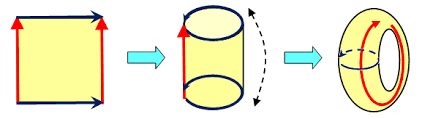
\includegraphics[scale=0.6]{pic/fig16}
\caption{圆柱形结构示意图}\label{fig15}
\end{figure}


\qquad 比如,我们考虑沿$y$方向取开边界条件,哈密顿量可以表示为
\begin{equation}
	\begin{aligned}
		H_{TI} &= \sum_{y,k_x}C^\dagger_{y}(k_x)[(h_0-2t\cos k_x)\sigma_3s_0 \\&+2\lambda_0\sin k_x\sigma_1s_0]C_{y}(k_x)
		+\sum_{y,k_x}[C^\dagger_{y}(k_x)\\&(-t\sigma_3s_0-i\lambda_0\sigma_2s_3)C_{y+1}(k_x)+h.c],
	\end{aligned}
\end{equation}

\begin{equation}
	\begin{aligned}
		H_{SC} &= \sum_{y,k_x,\sigma}d^\dagger_{y\sigma}(k_x)(-2t\cos k_x -\mu)d_{y\sigma}(k_x)\\
		&+\sum_{y,k_x}[d^\dagger_{y\uparrow}(k_x)(-2\Delta_0\cos k_x)d^\dagger_{y\downarrow}(-k_x)+h.c]
		\\&-t\sum_{y,k_x,\sigma}[d^\dagger_{y\sigma}(k_x)d_{y+1,\sigma}(k_x)+h.c]\\
		&+\Delta_0\sum_{y,k_x}[d^\dagger_{y\uparrow}(k_x)d^\dagger_{y+1,\downarrow}(-k_x)+h.c],
	\end{aligned}
\end{equation}
\begin{equation}
	H_I=-t_\perp\sum_{y,k_x,\alpha,\sigma}[c^\dagger_{y\alpha\sigma}(k_x)d_{y\sigma}(k_x)+h.c].
\end{equation}
\qquad 为了在实空间数值的研究马约拉纳拐角态,我们需要同时在$x$与$y$方向上取开边界条件。在这种情况下,哈密顿量在实空间的表达形式为
\begin{equation}
	\begin{aligned}
		H_{TI} &=-t\sum_{{\bf i}\alpha}(C_{{\bf i}}^\dagger \sigma_3s_0   C_{{\bf i}+\hat{\alpha}}+h.c.)+h_0\sum_{{\bf i}\tau}C_{{\bf i}}^\dagger \sigma_3s_0   C_{{\bf i}}
		\\&-\lambda_0\sum_{{\bf i}}(iC_{{\bf i}}^\dagger\sigma_1s_3C_{{\bf i}+\hat{x}}-iC_{{\bf i}}^\dagger\sigma_2s_0C_{{\bf i}+\hat{y}}+h.c.),
	\end{aligned}
\end{equation}
\begin{equation}
	\begin{aligned}
		H_{sc} &=-t\sum_{{\bf i}\alpha\sigma}(d_{{\bf i}\sigma}^\dagger d_{{\bf i}+\hat{\alpha},\sigma}+h.c.)-\mu\sum_{{\bf i}\sigma}d_{{\bf i}\sigma}^\dagger d_{{\bf i}\sigma}
		\\&+\sum_{\langle{\bf ij}\rangle}(\Delta_{\bf ij}d_{{\bf i}\uparrow}^\dagger d_{{\bf j}\downarrow}^\dagger+h.c.),
	\end{aligned}
\end{equation}

\begin{equation}
	H_{I}=-t_\perp \sum_{{\bf i}\tau\sigma}(c_{{\bf i}\tau\sigma}^\dagger d_{{\bf i}\sigma}+h.c.),
\end{equation}
对于$d$-波超导体配对,格点$\mathbf{j}$代表着格点$\mathbf{i}$的最近邻位置,$\Delta_\mathbf{ij}=\pm\Delta_0$,由于$d$-波配对$\pm$号依赖于$\langle\mathbf{ij}\rangle$是沿着$x$方向还是$y$方向。

\qquad 整个的哈密顿量可以被写成矩阵形式。在动量空间中它是一个$12\times 12$的矩阵$\hat{M}$,$H=\sum_{\mathbf{k}}\Psi_\mathbf{k}^\dagger\hat{M}\Psi_\mathbf{k}$。这里矢量$\Psi^\dagger_\mathbf{k}$表示为
\begin{equation}
\Psi^\dagger_{\bf k}=(C^\dagger_{\bf k},C_{-{\bf k}},d^\dagger_{{\bf k}\uparrow},d^\dagger_{{\bf k}\downarrow},d_{-{\bf k}\uparrow},d_{-{\bf k}\downarrow}).
\end{equation}
哈密顿量的矩阵形式$\hat{M}$可以表示为
\begin{equation}
\left[
\begin{array}{ccc}
M^{TI}(\mathbf{k}) & \mathbf{0}_{4\times 4} &M_1 \\
\mathbf{0}_{4\times 4} & -M^{TI}(\mathbf{-k}) & M_2 \\
M^{\dagger}_1 & M^{\dagger}_2 & M^{SC}(\mathbf{k})
\end{array}
\right],
\end{equation}
这里
\begin{equation}
M^{TI}(\mathbf{k})=\left[
\begin{array}{cccc}
h({\mathbf{k}}) & \lambda(\mathbf{k}) & 0 & 0 \\
\lambda(\mathbf{k})^* & -h({\mathbf{k}}) & 0 & 0 \\
0 & 0 & h({\mathbf{k}}) & -\lambda(\mathbf{k})^* \\
0 & 0 & -\lambda(\mathbf{k})^\dagger & -h({\mathbf{k}}),
\end{array}
\right]
\end{equation}
取 $\lambda(\mathbf{k})= 2\lambda_0\sin k_x- 2i\lambda_0\sin k_y$.

\begin{equation}
M^{SC}(\mathbf{k})=
\left[
\begin{array}{cccc}
\epsilon({\mathbf{k}}) & 0 & 0 & \Delta(\mathbf{k}) \\
0 & \epsilon({\mathbf{k}}) & -\Delta(\mathbf{k}) & 0 \\
0 & -\Delta(\mathbf{k}) & -\epsilon({\mathbf{k}}) & 0 \\
\Delta(\mathbf{k}) & 0 & 0 & -\epsilon({\mathbf{k}})
\end{array}
\right],
\end{equation}
\begin{equation}
M_1=-t_{\perp}\left[
\begin{array}{cccc}
1 & 0 & 0 & 0 \\
1 & 0 & 0 & 0 \\
0 & 1 & 0 & 0 \\
0 & 1 & 0 & 0
\end{array}
\right],\quad
M_2=-t_{\perp}\left[
\begin{array}{cccc}
0 & 0 & -1 & 0 \\
0 & 0 & -1 & 0 \\
0 & 0 & 0 & -1 \\
0 & 0 & 0 & -1
\end{array}
\right].
\end{equation}
在一个圆柱体结构且沿$y$方向取开边界条件,此时整个哈密顿量可以被写为$12N_y\times 12N_y$的矩阵形式$H=\sum_{k_x}\Psi^\dagger(k_x)\hat{M}(k_x)\Psi(k_x)$。$N_y$是沿$y$方向取开边界条件时所取的格点数目。矢量$\Psi^\dagger(k_x)$可以表示为
\begin{equation}
\Psi^\dagger(k_{x}) =(C^\dagger_1(k_x),C_{1}(k_x),\cdots,C^\dagger_{N_y}(k_x),C_{N_y}(k_x),d^\dagger_{1\uparrow}(k_x),\cdots,d_{N_y\downarrow}(k_x)).\label{b1}
\end{equation}

\qquad 在实空间中,哈密顿量矩阵$\hat{M}$大小为$N\times N$,这里$N=8N_1+4N_2$,$N_1,N_2$分别是实空间中2D拓扑绝缘体和$d$-波超导体的格点数目。矢量$\Psi^\dagger$表示为
\begin{eqnarray}
\Psi^\dagger =(C^\dagger_1,C_{1},\cdots,C^\dagger_{N_1},C_{N_1},d^\dagger_{1\uparrow},\cdots,d_{N_2\downarrow}).\label{b2}
\end{eqnarray}
方程(\ref{b1})中的矢量$C^\dagger_i(k_x)$和方程(\ref{b2})中的$C^\dagger_i$是矢量$C^\dagger_\mathbf{k}$的傅里叶变换。

\qquad 通过对哈密顿量矩阵进行对角化,我们可以得到推迟格林函数矩阵$\hat{G}$,其矩阵元表示为
\begin{equation}
G_{ij}(E)=\sum_n\frac{u_{in}u^{*}_{jn}}{E-E_n+i\Gamma}.
\end{equation}
这里$u_{in}$ 和 $E_n$分别代表着矩阵的本征矢量和本征值。

\qquad 在动量空间中,2D拓扑绝缘体层的谱函数可以通过格林函数计算
\begin{equation}
A({\bf k},E)=-\frac{1}{\pi}\sum^4_{p=1}\mathrm{Im} G_{pp}({\bf k},E).
\end{equation}

\qquad 对于一个圆柱体结构,谱函数可以通过下面公式计算
\begin{equation}
A_{y}(k_{x},\omega)=-\frac{1}{\pi}\sum_{p=1}^{4}\mathrm{Im} G_{m+p,m+p}(k_x,\omega),
\end{equation}
这里 $m = 8(i_y-1)$。

\qquad 对于轨道$\mathbf{\tau}$通过近邻效应诱导的配对项可以通过平均场序参量来研究,表达为
\begin{equation}
\Delta_\tau({\bf k})=\langle c^\dagger_{{\bf k}\tau\uparrow}c^\dagger_{-{\bf k}\tau\downarrow}\rangle=\sum_n{u^{*}_{\tau,n}({\bf k})u_{\tau+6,n}({\bf k})}f(E_n),
\end{equation}
这里$f(x)$代表费米分布函数。

\qquad 在实空间中,轨道$\mathbf{\tau}在$格点$i$和$j$上的有效配对序参量表达式为
\begin{equation}
\Delta^\tau_{ij}=\sum_nu^{*}_{h(i),n}u_{h(j)+6,n}f(E_n),
\end{equation}
这里 $h(i)=\tau+8(i-1)$。

\qquad 我们可以对轨道$\mathbf{\tau}$定义一个位置以来的$d$-波配对
\begin{equation}
\Delta^\tau_i=\mid \Delta^\tau_{i,i+\hat{x}}+\Delta^\tau_{i,i-\hat{x}}
-\Delta^\tau_{i,i+\hat{y}}-\Delta^\tau_{i,i-\hat{y}}\mid.
\end{equation}
在系统的边界上,$\Delta_i^\tau$表示为
\begin{equation}
\Delta^\tau_i=\mid 2(\Delta^\tau_{i,i+\hat{\alpha}}+\Delta^\tau_{i,i-\hat{\alpha}}) \mid  \qquad (\alpha=x,y).
\end{equation}

\qquad 在2D拓扑绝缘体的格点$i$上的局域电子态密度(LDOS)可以通过实空间中的格林函数计算
\begin{equation}
\rho_i(E)=-\frac{1}{\pi}\sum^4_{p=1}\mathrm{Im} G_{m+p,m+p}(E).
\end{equation}
这里 $m=8(i-1)$。

\qquad 在接下来的计算中,我们取跃迁常数$t$作为能量单位(从高温超导体的带宽可以估计出$t=0.17eV$),其他的参数设置如下;$\lambda_0=0.5$, $h_0=3$, $\mu=-0.3$, $\Delta_0=0.2$, $t_\perp=0.8$,$\Gamma=0.01$.
%============================================
\subsection{运动方程}
\qquad 对任意两个算符$A$与$B$组成的函数,在海森堡绘景中
\begin{equation}
\begin{aligned}
G_r(t,t^{'})&=-\frac{i}{\hbar}\theta(t-t^{'})\langle\left[A(t),B(t^{'})\right]_\pm\rangle\\
&=\left\{
\begin{array}{cc}
-\frac{i}{\hbar}(\langle A(t)B(t^{'})\rangle\pm\langle B(t^{'})A(t)\rangle)\quad (t>t^{'})\\
0\quad(t<t^{'})
\end{array}
\right.\\
&=\langle\langle A(t);B(t^{'})\rangle\rangle_r\label{eom1}
\end{aligned}
\end{equation}
这里泊松括号的下标$\pm$是为了方便这样标记的,当$A$与$B$是费米子型算符时,满足反对易关系,此时取$+$号,而对于玻色子型算符,则满足对易关系,此时取$-$号。在公式(\ref{eom1})中$\langle\dots\rangle$代表统计平均,对于正则系综
\begin{equation}
\langle A\rangle=Z^{-1}\mathrm{Tr}(e^{-\beta H}A),\quad Z=\mathrm{Tr}(e^{-\beta H}),\quad\beta=(k_BT)^{-1}
\end{equation}
由于算符乘积就迹具有轮换不变性
\begin{equation}
\mathrm{Tr}(ABC)=\mathrm{Tr}(CAB)=\mathrm{Tr}(BCA)
\end{equation}
则可以推导出
\begin{equation}
\begin{aligned}
\langle A(t)B(t^{'})\rangle&=Z^{-1}\mathrm{Tr}(E^{-\beta H}e^{\frac{i}{\hbar}Ht}Ae^{-\frac{i}{\hbar}H(t-t^{'})}Be^{-\frac{i}{\hbar}Ht^{'}})\\
&=Z^{-1}\mathrm{Tr}(e^{-\beta H}e^{\frac{i}{\hbar}H(t-t^{'})}Ae^{-\frac{i}{\hbar}H(t-t^{'})}B)\\
&=Z^{-1}\mathrm{Tr}\left[e^{-\beta H}A(t-t^{'})B\right]\\
&=\langle A(t-t^{'})B(0)\rangle
\end{aligned}
\end{equation}
同理也可以证明
\begin{equation}
\langle B(t^{'}A(t))\rangle=\langle B(0)A(t-t^{'})\rangle
\end{equation}
于是双时格林函为
\begin{equation}
\begin{aligned}
G_r(t,t^{'})&=-\frac{i}{\hbar}\theta(t-t^{'})\langle\left[A(t),B(t^{'})\right]_\pm\rangle\\
&=-\frac{i}{\hbar}\langle\left[A(t-t^{'}),B(0)\right]_\pm\\
&=G_r(t-t^{'})
\end{aligned}
\end{equation}
这说明$G_r$只是时间差$(t-t^{'})$的函数。我们可以简单的令$t^{'}=0$,并令$t$代表时间差,则格林函数的定义就可以简化为
\begin{equation}
G_r(t)\equiv\langle\langle A(t);B\rangle\rangle_r=-\frac{i}{\hbar}\theta(t)\langle\left[A(t),B\right]_\pm\rangle\label{gf1}
\end{equation}
其中$B=B(0)$,而
\begin{equation}
A(t)=e^{\frac{i}{\hbar}H t}Ae^{-\frac{i}{\hbar }H t}
\end{equation}
$G_r(t)$的傅里叶变换为
\begin{equation}
G_r(t)=\frac{1}{2\pi}\int_{-\infty}^{\infty}d\omega G_r(\omega)e^{-i(\omega+i\eta)t}\qquad(\eta=+0)
\end{equation}
其逆变换为
\begin{equation}
G_r(\omega)=\int_{-\infty}^{\infty}dtG_r(t)e^{i(\omega+i\eta)t}\equiv\langle\langle A|B\rangle\rangle_{\omega+i\eta}\label{gr}
\end{equation}
在实际的运算中,更多讨论的是格林函数$G_r(\omega)$的性质。

\qquad 对于有限温度,各种本征态$|n\rangle$均以概率$Z^{-1}e^{\beta E_n}$出现,此时公式(\ref{gf1})中的$\langle(\dots)\rangle$不再是基态平均$\langle n|(\dots)|n\rangle$,而应该取统计平均$Z^{-1}\sum_ne^{-\beta E_n}\langle n|(\dots)|n\rangle$,则可以将(\ref{gf1})表示为
\begin{equation}
-\frac{i}{\hbar}\theta(t)Z^{-1}\sum_{n,m}e^{-\beta E_n}\{\langle n|A|m\rangle\langle m|B|\rangle e^{i\omega_{nm}t}\pm\langle n|B|m\rangle\langle m|A|n\rangle e^{-i\omega_{nm}t}\}
\end{equation}
其中$\omega_{nm}\equiv(E_n-E_m)$,再对上式中的第一项做变量替换$n\leftrightarrow m$,即可以得到温度$T>0$时的$G_r(t)$为
\begin{equation}
G_r(t)=-\frac{i}{\hbar}\theta(t)Z^{-1}\sum_{n,m}e^{-\beta E_n}\langle n|B|m\rangle\langle m|A|n\rangle\times e^{-\frac{i}{\hbar}(E_n-E_m)t}(e^{\beta(E_n-E_m)}\pm 1)\label{gf2}
\end{equation}
通过对(\ref{gf2})做傅里叶变换,即可得到频率空间的表示
\begin{equation}
\begin{aligned}
G_r(\omega)&=Z^{-1}\sum_{n,m}e^{-\beta E_n}\langle n|B|m\rangle\langle m|A|n\rangle\times\frac{e^{\beta(E_n-E_m)}\pm 1}{\hbar\omega-(E_n-E_m)+i\eta}\\
&\equiv\langle\langle A|B\rangle\rangle_{\omega+i\eta}\label{gf3}
\end{aligned}
\end{equation}
谱函数表示为
\begin{equation}
\begin{aligned}
A(\omega)&\equiv-\frac{1}{\pi}\mathrm{Im}G_r(\omega)\\
&=Z^{-1}\sum_{n,m}e^{-\beta E_n}\langle n|B|m\rangle\langle  m|A|n\rangle(e^{\beta\hbar\omega_{nm}}\pm 1)\delta\left[\hbar\omega-(E_n-E_m)\right]\\
&=Z^{-1}\sum_{n,m}\langle n|B|m\rangle\langle  m|A|n\rangle(e^{-\beta E_m}\pm e^{-\beta E_n})\delta\left[\hbar\omega-(E_n-E_m)\right]
\end{aligned}
\end{equation}

\qquad 推迟格林函数$\langle\langle A|B\rangle\rangle_{\omega+i\eta}$的极点在下半复平面,它只是上半复平面的解析函数,如果将(\ref{gr})中的$i\eta$换成$-i\eta$则可以定义一个在下半复平面的解析函数
\begin{equation}
\langle\langle A|B\rangle\rangle_{\omega-i\eta}\equiv Z^{-1}\sum_{n,m}e^{-\beta E_n}\langle n|B|m\rangle\langle m|A|n\rangle\times \frac{e^{\beta(E_n-E_m)}\pm 1}{\hbar\omega-(E_n-E_m)-i\eta}=G_a(\omega)\label{gf4}
\end{equation}
它的极点在上半平面,再对$G_a(\omega)$做傅里叶变换
\begin{equation}
\begin{aligned}
G_a(t)&=\frac{1}{2\pi}\int_{-\infty}^{\infty}d\omega G_a(\omega)e^{-i(\omega-i\eta)t}\quad(\eta=+0)\\
&=-\frac{i}{\hbar}\theta(-t)\langle\left[A(t),B\right]_\pm\rangle\equiv\langle\langle A(t);B\rangle\rangle_a\\
&=\left\{
\begin{array}{cc}
0\qquad(t>0)\\
\frac{i}{\hbar}\{\langle A(t)B\rangle\pm\langle BA(t)\rangle\}\qquad(t<0)
\end{array}
\right.
\end{aligned}
\end{equation}
这里所求的的时间关联函数是逆时序传播的,代表超前格林函数,因此用$G_a(t)$与$G_a(\omega)$表示。

\qquad 利用$G_r(\omega)$与$G_a(\omega)$可以定义包含上、下半复平面在内的全格林函数
\begin{equation}
\begin{aligned}
G(\omega)&\equiv\langle\langle A|B\rangle\rangle_\omega\\
&=Z^{-1}\sum_{n,m}e^{-\beta E_n}\langle n|B|m\rangle\langle m|A|n\rangle\frac{e^{\beta(E_n-E_m)}\pm 1}{\hbar\omega-(E_n-E_m)}\\
&=\left\{
\begin{array}{cc}
G_r(\omega)\qquad(\textrm{上半复平面})\\
G_a(\omega)\qquad(\textrm{下半复平面})
\end{array}\right.\label{gf5}
\end{aligned}
\end{equation}
这里$\omega$为复量。

\qquad 利用公式(\ref{gf5})中定义的全格林函数$G(\omega)$,做傅里叶变换即可以得到响应的全时格林函数
\begin{equation}
\begin{aligned}
G(t)&\equiv\frac{1}{2\pi}\int_{-\infty}^{\infty}d\omega e^{-\omega t}G(\omega)\equiv\langle\langle A(t);B\rangle\rangle\\
&=\left\{
\begin{array}{cc}
-i\theta(t)\langle \left[A(t),B\right]_\pm\rangle=G_r(t)\\
i\theta(-t)\langle \left[A(t),B\right]_\pm\rangle=G_a(t)\\
\end{array}
\right.\label{gf6}
\end{aligned}
\end{equation}
这里$G(t>0)$代表推迟格林函数,$G(t<0)$则表示超前格林函数。$A(t)$为海森堡绘景中的算符
\begin{equation}
A(t)=e^{iHt}Ae^{-iHt}\label{hs1}
\end{equation}
这里选取自然单位制$\hbar=1$,从方程(\ref{gf5})出发,利用海森堡运动方程
\begin{equation}
i\frac{dA(t)}{dt}=\left[A(t),H\right]=A(t)H-HA(t)
\end{equation}
对公式(\ref{gf6})求时间的导数
\begin{equation}
\begin{aligned}
i\frac{d}{dt}\langle\langle A(t);B\rangle\rangle&=\delta(t)\langle \left[A(t),B\right]_\pm\rangle\mp i\theta(\pm t)\langle\left[\left[A(t),H\right],B\right]_\pm\rangle\\
&=\delta(t)\langle\left[A,B\right]_\pm+\langle\langle\left[A(t),H\right];B\rangle\rangle\label{gf7}
\end{aligned}
\end{equation}
再利用
\begin{equation}
\begin{aligned}
\delta(t)&=\frac{1}{2\pi}\int_{-\infty}^{\infty}d\omega e^{-i\omega t}\\
i\dot{G}(t)&=\frac{1}{2\pi}\int_{-\infty}^{\infty}d\omega G(\omega)e^{-i\omega t}\\
&=\frac{1}{2\pi}\int_{-\infty}^{\infty}d\omega \langle\langle A|B\rangle\rangle_\omega e^{-i\omega t}\label{gf8}
\end{aligned}
\end{equation}
在(\ref{gf8})中出现的高阶格林函数也可以做傅里叶变换,用复平面内的$\omega$分量表示为
\begin{equation}
\langle\langle\left[A(t),H\right];B\rangle\rangle=\frac{1}{2\pi}\int_{-\infty}^{\infty}d\omega \langle\langle\left[A,H\right]|B\rangle\rangle_\omega e^{-i\omega t}\label{gf9}
\end{equation}
将(\ref{gf8}-\ref{gf9})代入(\ref{gf7})中,可以求得在复平面$\omega$上的格林函数运动方程为
\begin{equation}
\omega\langle\langle A|B\rangle\rangle_\omega=\langle\left[A,B\right]_\pm\rangle+\langle\langle\left[A,H\right]|B\rangle\rangle_\omega\label{gf10}
\end{equation}
上式(\ref{gf10})右边的的$\langle\langle\left[A,H\right]|B\rangle\rangle_\omega$是高阶格林函数,它所满足的运动方程仍然为(\ref{gf10}),

















